
\chapter{Telas da Aplicação}
\label{chap:telas}

Para acessar a aplicação, além de utilizar contas no Facebook ou Google, é possível criar uma conta diretamente na aplicação, ilustrado na Figura \ref{img:tela-criacao}

\begin{figure}[H]
    \centering
    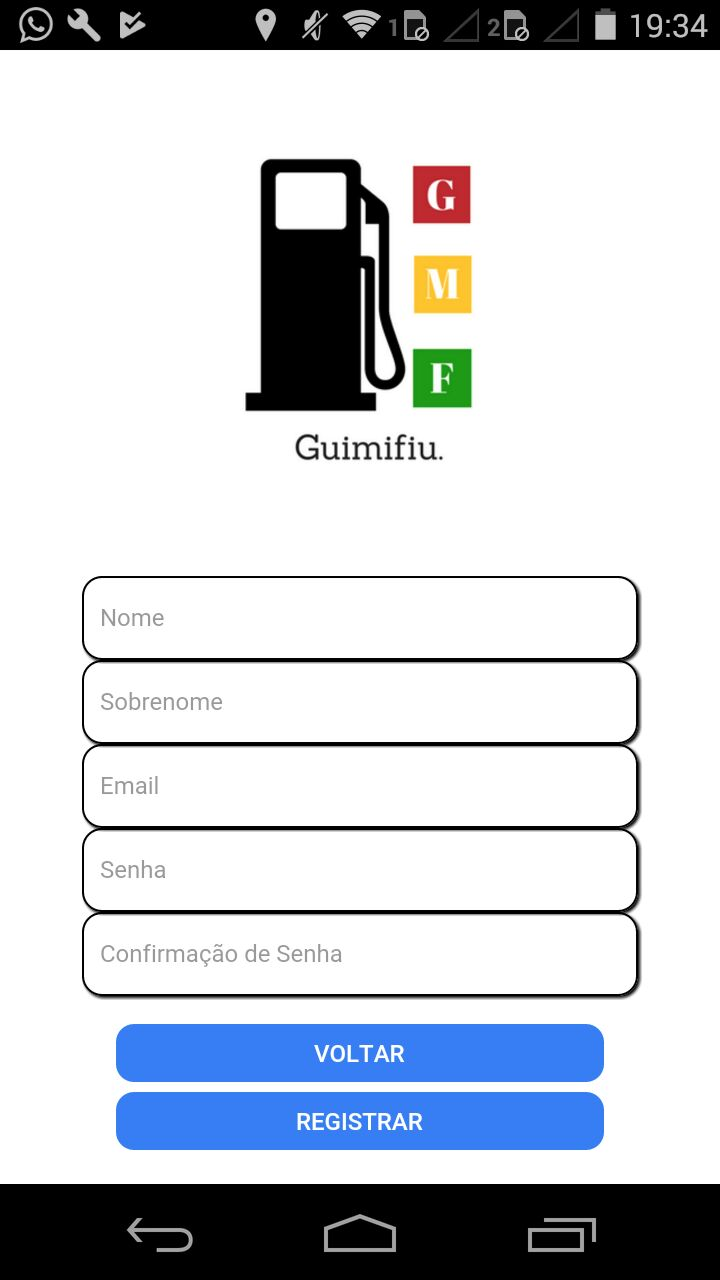
\includegraphics[scale=0.2]{figuras/tela-criacao.jpeg}
    \caption[Tela de criação de conta]{Tela de criação de conta. Fonte: autores}
    \label{img:tela-criacao}
\end{figure}

A aplicação pode mostrar os detalhes de um posto de combusível específico, assim como iniciar uma rota para chegar nele, como mostra a Figura \ref{img:tela-detalhamento}

\begin{figure}[H]
    \centering
    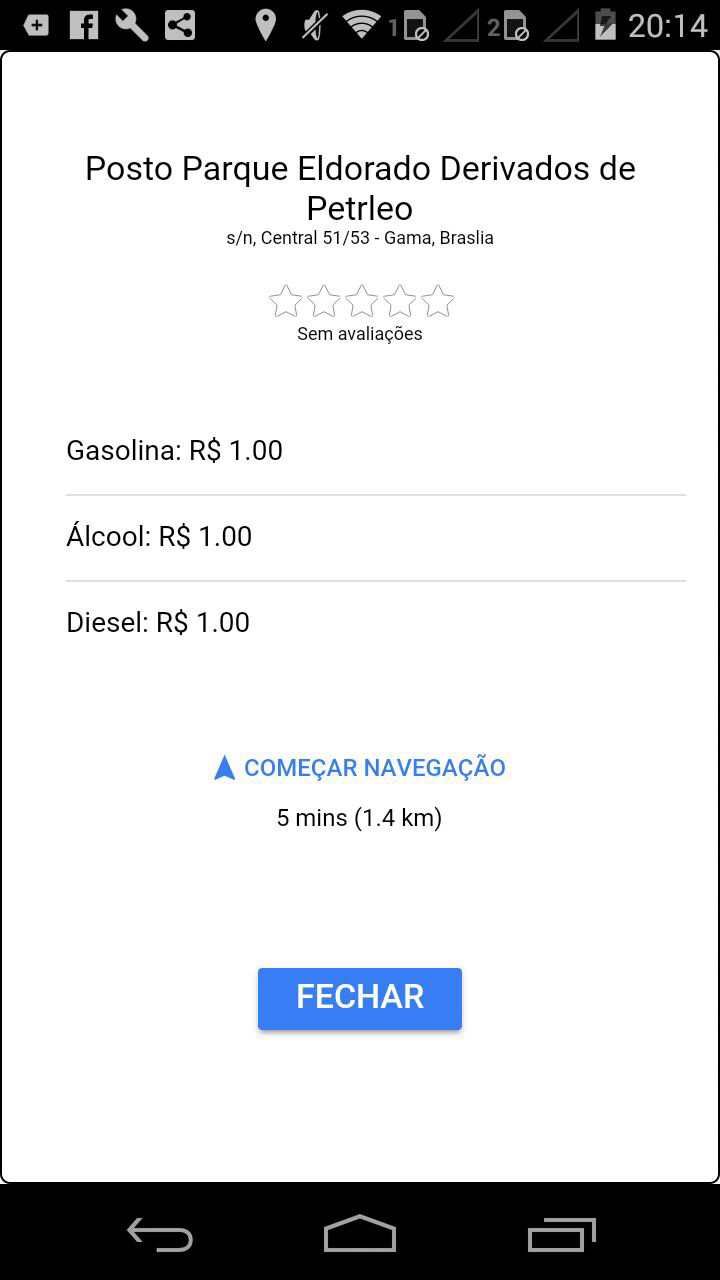
\includegraphics[scale=0.2]{figuras/app_final_4.jpg}
    \caption[Tela de detalhes do posto de combustível na rota]{Tela de detalhes do posto de combustível na rota. Fonte: autores}
    \label{img:tela-detalhamento}
\end{figure}

É possível também inserir um endereço para o aplicativo planejar uma rota e mostrar todos os postos de combustíveis perto daquela rota, como ilustra a Figura \ref{img:buscando_localizacoes}.

\begin{figure}[H]
    \centering
    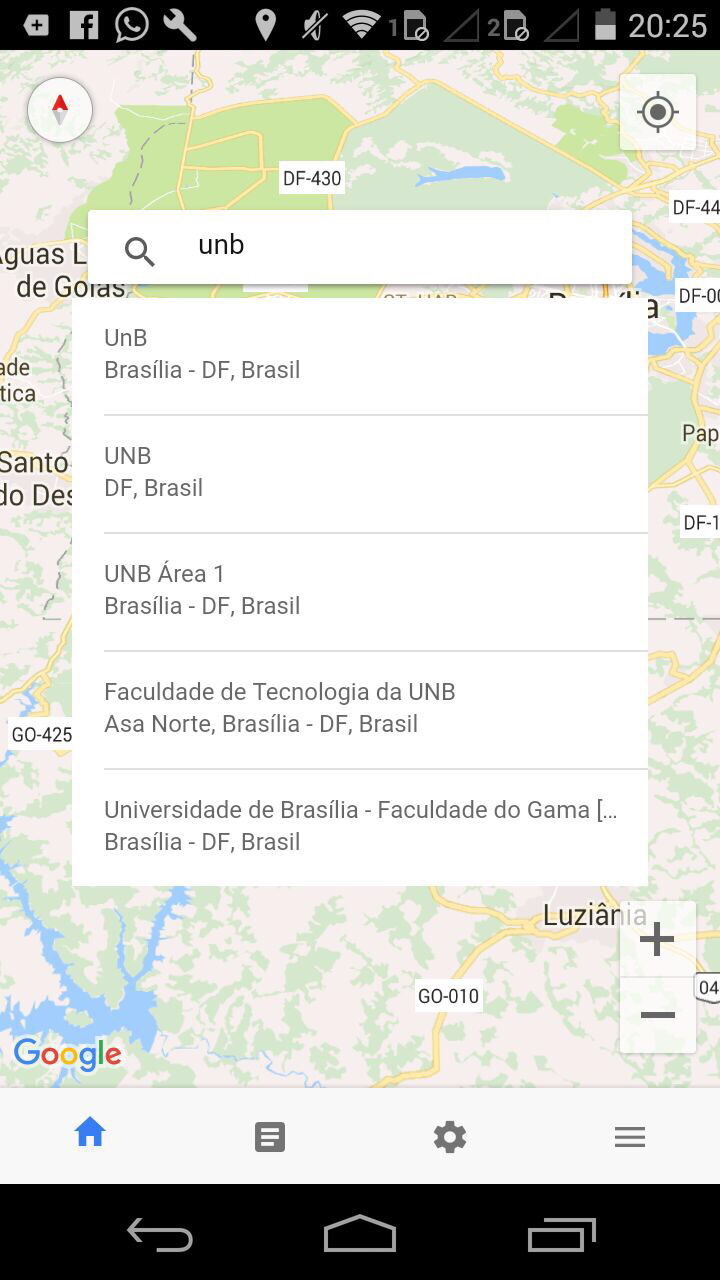
\includegraphics[scale=0.2]{figuras/app_3.jpg}
    \caption[Buscando localizações]{Buscando localizações. Fonte: autores}
    \label{img:buscando_localizacoes}
\end{figure}
